\subsection{Setting}\label{sw:sec:setting}

Fix a $d$-level system $A$ with Hamiltonian $H$, an inverse temperature $\beta=1/\kB T>0$, and the Gibbs state $\gamma=e^{-\beta H}/\Tr e^{-\beta H}$. Entropies and logarithms are base two. A channel $\Phi$ on $A$ is \emph{time-covariant} if $\Phi(e^{-iHt}\rho\, e^{iHt})=e^{-iHt}\Phi(\rho)e^{iHt}$ for all $t$. Energy-conserving dynamics without an external phase reference can only implement such channels~\cite{Lostaglio15,FBB21}.

\paragraph{The device.} An implementation consists of a controller $C$, a battery $B$ and a reservoir $R$. The controller holds all hardware: memory, clocks, catalysts and any work registers not charged to the battery. The reservoir is a finite collection of cells, each with its own Hamiltonian. All cells are declared in advance, including those used only late or only after the last output. They start in their Gibbs states at inverse temperature $\beta$, independent of each other and of everything else. The initial state is $\alpha_C\otimes\zeta_B\otimes\gamma_R$, with an additive Hamiltonian $H_C+H_B+H_R$. Every operation is a unitary that commutes with the total Hamiltonian of the systems it acts on. Measurements and records are part of the dilation and are counted. No other resource is free: there is no external coherence, no Gibbs-preserving map supplied as a black box, and no initial correlation between $C$, $B$ and $R$. The battery is \emph{stationary} if $\zeta_B$ commutes with $H_B$, as an energy eigenstate does. A stationary battery holds no phase reference, so every clock of the device is then in its controller.

\paragraph{Real-time operation.} The device serves $n$ rounds. In round $t$ an input system arrives, the device acts on it together with its internal systems, and the output is released. Input $t+1$ is supplied only after output $t$ has left. Between rounds, and after the last one, the device may act on its internal systems as it likes. It never acts again on a delivered output. The inputs come from an observer who may choose them adaptively and keep quantum references. The \emph{error} $\varepsilon$ is the largest trace distance $\tfrac12\|\cdot\|_1$, over all such observers, between the final state of the observer's systems with the device and with $n$ ideal uses of $\Phi$. This is the distance between strategies of~\cite{Chiribella08,GutoskiWatrous07}.

\paragraph{Batch operation.} For comparison, a batch implementation may hold all outputs until the end. Its error is the half diamond distance to $\Phi^{\otimes n}$, the criterion of~\cite{FBB21}.

\paragraph{Work.} The controller must return. For the constructions of time-covariant channels it returns exactly to $\alpha_C$, independent of all other systems, and Theorem~\ref{sw:thm:clock} relaxes this for the other channels; for the lower bounds it is enough that its free energy returns up to $o(n)$. The battery is mechanical: work is its mean loss of energy, and its entropy changes by $o(n)$, so it cannot hide a second bath. Work is \emph{deterministic} when the battery starts in an energy eigenstate, ends, with probability tending to one for every observer, in a fixed energy eigenstate, and its mean energy differs from that eigenvalue by $o(n)$ (a signed mean deviation; the general law of Section~\ref{sec:law} and Part~\ref{app:batch} use the stronger mean absolute deviation $\Tr|H_B-E|\rho_B$, and say so); this is the mechanical counterpart of the information battery checked by a projector in~\cite{FR18,FBB21}. The last clause matters only for a controller that returns approximately (Section~\ref{sw:sec:free}): it prevents a broad reference from lending the device energy that the battery repays in one rare, large event. In the fixed-error statement of Theorem~\ref{sw:thm:law} the controller also starts in a thermal state (Remark~\ref{sw:rem:thermal-controller}). For a family of implementations with error $\varepsilon_n\to0$, the \emph{work rate} is $\limsup_n W_n/(n\kB T\ln 2)$, in bits per use. The optimal real-time and batch rates are the infima over such families.

These rates allow reservoirs, controllers and running times of any finite size. They describe what is possible in principle, not an efficient or autonomous engine.

\begin{remark}[Battery models]\label{sw:rem:battery}
Faist, Berta and Brand\~ao count work as purity in an information battery~\cite{FR18,FBB21}; we use a mechanical battery, so that work is energy. Our lower bounds are statements about the free energy drawn from battery and controller (Lemma~\ref{sw:lem:accounting}), so they hold in both conventions. We quote $\Tcap$ as the batch benchmark in their convention.
\end{remark}

\begin{definition}[Real-time entropy cost]\label{sw:def:rtcost}
Let $\psi_\rho$ purify a full-rank input $\rho$ with reference $Q$, and let $\chi_\rho=(\mathrm{id}_Q\otimes\Phi)(\psi_\rho)$ on $QO$. For $\varepsilon>0$ let
\[
s_{\rho,\varepsilon}(\Phi)=\inf S(QO|F)_\sigma,
\]
over finite systems $F$ and states $\sigma_{QOF}$ with $\sigma_{QF}=\rho^{T}\otimes\sigma_F$ and $\tfrac12\|\sigma_{QO}-\chi_\rho\|_1\le\varepsilon$. The \emph{real-time entropy cost} is $s_\rho(\Phi)=\lim_{\varepsilon\downarrow0}s_{\rho,\varepsilon}(\Phi)$.
\end{definition}

Think of $F$ as a purification of everything the device holds when the input arrives. The product condition $\sigma_{QF}=\rho^T\otimes\sigma_F$ says that none of it carries information about the fresh input. After the round, $S(QO|F)$ equals the increase in the entropy of the device's internal state (Lemma~\ref{sw:lem:accumulation}). So $s_\rho(\Phi)$ is the least entropy that one use on input $\rho$ must add to a device that did not know the input in advance. Since $S(QO|F)\ge S(Q)-S(O)$ whenever $QF$ is a product, $s_\rho(\Phi)\ge S(\rho)-S(\Phi(\rho))$. At zero Hamiltonian, $\Trt(\Phi)=\sup_\rho s_\rho(\Phi)$ is the purity cost of real-time operation of our earlier work, where it is written $\kappa(\Phi)$~\cite{Memory,ImmediateDelivery,Douglas26closed}.


\begin{lemma}[Pointwise smoothing~{\cite[Thm.~4.1, Cor.~4.3]{Douglas26closed}}]\label{sw:lem:smoothing}
For every channel $\Phi$ and every full-rank input $\rho$,
\[
s_\rho(\Phi)=\lim_{\varepsilon\downarrow0}s_{\rho,\varepsilon}(\Phi)=\inf\bigl\{S(E')-S(\tau):(U,\tau)\ \text{a finite exact dilation of }\Phi\bigr\}.
\]
\end{lemma}
\begin{proof}
An exact dilation is an exact extension, which gives $\le$ at every $\varepsilon$. For the converse an $\varepsilon$-feasible extension lifts, through the purification $\psi_\rho$, to a dilation of a channel within diamond distance $\varepsilon/\lambda_{\min}(\rho)$ of $\Phi$ with the same objective, and the support repair of~\cite[Thm.~4.1 and Cor.~4.3]{Douglas26closed} replaces it by an exact dilation of $\Phi$ whose objective differs by a quantity that tends to zero with $\varepsilon$ and depends only on $\Phi$ and $\rho$, not on the size of the bath. Letting $\varepsilon\to0$ gives $\ge$.
\end{proof}
At a fixed input this value is a known entropy functional. Every exact extension arises from a channel applied to the environment $E$ of a Stinespring purification $\psi_{QOE}$ of $\chi_\rho$, and the product condition says that the channel's output carries no information about $Q$. Hence $s_\rho(\Phi)=S(\chi_\rho)-P_{\mathrm q}(0)$, where $P_{\mathrm q}$ is the quantum privacy funnel of Datta, Hirche and Winter~\cite[Sec.~V, Eq.~(22)]{DattaHircheWinter19}, with their $X=E$, $Y=Q$ and $R=O$, evaluated at zero leakage~\cite[Eq.~(1.3), Cor.~4.3]{Douglas26closed}; its supremum runs over all finite auxiliary dimensions. Datta, Hirche and Winter doubted that the funnel describes an asymptotic rate, since even its classical version is not additive over i.i.d.\ blocks. In real time no block coding is possible, and at zero Hamiltonian the rate of Theorem~\ref{sw:thm:law} is the supremum of $S(\chi_\rho)-P_{\mathrm q}(0)$ over full-rank inputs; Lemma~\ref{sw:lem:smoothing} supplies the continuity at vanishing error that this identification needs.

There is a second way to read $s_\rho$. A dilation of $\Phi$ is a unitary $U$ on the input and a bath in state $\tau$ with $\Phi(\rho)=\Tr_E U(\rho\otimes\tau)U^*$. On input $\rho$ it ends with the output $O$ and the bath $E'$ in a joint state, and conservation of entropy gives $S(E')-S(\tau)=S(\rho)-S(\Phi(\rho))+I(O{:}E')$. By Lemma~\ref{sw:lem:smoothing}, the real-time entropy cost is the infimum of $S(E')-S(\tau)$ over exact finite dilations, input by input. Hence~\eqref{sw:eq:mutual} holds with
\[
m_\rho(\Phi)=\inf\bigl\{\,I(O{:}E')_\rho:\ (U,\tau)\ \text{a finite dilation of}\ \Phi\,\bigr\}.
\]
The batch cost is the same expression with $m_\rho=0$. A batch device approaches it by erasing its baths with the outputs as side information~\cite[Sec.~7]{FBB21}. This works up to an error that can be made arbitrarily small for large $n$; at zero error it can fail completely (Theorem~\ref{sw:thm:werner}).

\subsection{The real-time work law}\label{sw:sec:law}

The lower bound comes from two facts: a bookkeeping identity that holds for every implementation, and a bound on how much entropy each real-time round must add to the device. The upper bound is a construction. Section~\ref{sw:sec:fixed-error} upgrades the lower bound to every fixed error.

\subsubsection{Bookkeeping}

Write $D=CBR$ for everything except the inputs and outputs, and let $A=S(D_{\mathrm{fin}})-S(D_{\mathrm{init}})$ be the entropy it gains. Let $\Delta E_{\mathrm{sys}}$ be the total energy delivered in the outputs minus the total energy taken from the inputs. Measure the free energy drawn from the battery and the controller in units of $\kB T\ln2$:
\[
w=\frac{F(\zeta_{\mathrm{init}})-F(\zeta_{\mathrm{fin}})+F(\alpha_{\mathrm{init}})-F(\alpha_{\mathrm{fin}})}{\kB T\ln 2},\qquad F(x)=\Tr(H x)-\kB T\ln2\,S(x).
\]

\begin{lemma}[Accounting identity]\label{sw:lem:accounting}
For every implementation in the model of Section~\ref{sw:sec:setting},
\[
w=A+\tfrac{\beta}{\ln2}\,\Delta E_{\mathrm{sys}}+D(R_{\mathrm{fin}}\|\gamma_R)+I(C{:}B{:}R)_{\mathrm{fin}},
\]
where $I(C{:}B{:}R)=S(C)+S(B)+S(R)-S(CBR)$ is the total correlation. In particular $w\ge A+\beta\Delta E_{\mathrm{sys}}/\ln2$.
\end{lemma}

\begin{proof}
Energy conservation gives $\Delta E_C+\Delta E_B+\Delta E_R+\Delta E_{\mathrm{sys}}=0$. For the reservoir, $S(R_{\mathrm{fin}})-S(\gamma_R)=\beta\Delta E_R/\ln2-D(R_{\mathrm{fin}}\|\gamma_R)$. Since $C$, $B$ and $R$ start independent, $A=\Delta S_C+\Delta S_B+\Delta S_R-I(C{:}B{:}R)_{\mathrm{fin}}$. Substituting into $w=\Delta S_B+\Delta S_C-\beta(\Delta E_B+\Delta E_C)/\ln2$ gives the identity.
\end{proof}

This is multipartite finite-reservoir Landauer bookkeeping~\cite{EspositoLindenbergVandenBroeck10,ReebWolf14}. Correlations with the observer do not enter, because the identity concerns only the device. A reservoir cell that is set aside can be kept in $R$ and left alone, so discarding never helps. Correlations that the controller keeps with past outputs, and catalysts it returns at the end, only add to $w$ through the last two terms.

\subsubsection{What each round must leave behind}

\begin{lemma}[Causal accumulation]\label{sw:lem:accumulation}
Suppose the error is at most $\varepsilon$, and the observer feeds each round one half of a fresh purification $\psi_\rho$ of a full-rank state $\rho$, keeping all references. Then in every round the entropy of the device rises by at least $s_{\rho,\varepsilon}(\Phi)$, so $A\ge n\,s_{\rho,\varepsilon}(\Phi)$.
\end{lemma}

\begin{proof}
Let $D_t$ be the device before round $t$ and let $F_t$ purify it; $F_t$ contains the earlier references and outputs. The fresh pair $Q_tS_t$ is independent of $D_tF_t$, and the round acts on $S_tD_t$ only, so $Q_tF_t$ stays a product. After the round the global state is pure, which gives $S(D_{t+1})-S(D_t)=S(Q_tO_t|F_t)$. The observer's state $Q_tO_t$ is within $\varepsilon$ of $\chi_\rho$, so this extension is feasible in Definition~\ref{sw:def:rtcost} and $S(Q_tO_t|F_t)\ge s_{\rho,\varepsilon}(\Phi)$. Operations on the device between rounds are unitary on $D$ and preserve its entropy, so the increments add up.
\end{proof}

The device's memory may be correlated with every earlier output; the lemma allows that. What it rules out is a memory that already knows the next input.

\subsubsection{The lower bound}

Each delivered output is within $\varepsilon$ of $\Phi(\rho)$, so its energy is within $\varepsilon\,\mathrm{span}(H)$ of $\Tr H\Phi(\rho)$, where $\mathrm{span}(H)$ is the difference between the largest and smallest eigenvalues. Combining the two lemmas with the same input $\rho$,
\begin{equation}\label{sw:eq:converse}
w\ \ge\ n\Bigl[s_{\rho,\varepsilon}(\Phi)+\tfrac{\beta}{\ln2}\Tr H\bigl(\Phi(\rho)-\rho\bigr)-\tfrac{\beta\varepsilon}{\ln2}\,\mathrm{span}(H)\Bigr]
\end{equation}
for every full-rank $\rho$. For a mechanical battery the actual work is $\kB T\ln2\,(w-\Delta S_B)$ when the controller returns, and $\Delta S_B=o(n)$. Letting $\varepsilon\to0$ and taking the supremum over $\rho$ gives the lower half of Theorem~\ref{sw:thm:law}. Neither time covariance nor a known horizon is used: the lower bound holds for every channel, and for any controller, including one that carries a phase reference. Recovery after the last output does not help either, since every reservoir cell used for it is already part of $D$.

\subsubsection{The construction}

The matching construction has three layers (Appendix~\ref{sw:app:construction}).

\emph{A real-time dilation.} For every $\eta>0$ there is a finite dilation of $\Phi$, a unitary $U$ acting on the input and a bath in state $\tau$, whose cost $\sup_\rho[S(\text{bath output})-S(\tau)+\beta\Tr H(\Phi(\rho)-\rho)/\ln2]$ is within $\eta$ of $\Trt(\Phi)$. This uses the pointwise smoothing identity of Lemma~\ref{sw:lem:smoothing} together with a minimax argument; the energy term is the same for every exact dilation.

\emph{Paying for entropy and energy together.} Running the dilation $n$ times, with a fresh bath copy each round, leaves the used baths in a state supported, up to exponentially small weight, on a subspace whose Gibbs weight is controlled by $\Trt(\Phi)+\eta$ bits per round. A single energy register records the total energy exchanged with the system. A positive-operator inequality, which survives arbitrary correlations between the baths, the register, the references and adaptively chosen inputs, charges entropy and energy on the same input. This plays the role of the universal conditional and relative typical operator of Faist, Berta and Brand\~ao, which also counts entropy against energy and serves every input type at once~\cite{FBB19}, \cite[Sec.~6]{FBB21}; here the universality comes instead from a single dilation chosen by the minimax argument and one operator inequality. Time covariance is used here: it lets an energy-conserving lift of $U$ reproduce the whole adaptive experiment exactly.

\emph{Paying the work.} An energy-conserving converter between two subspaces of given Gibbs weight moves a battery by the logarithm of their ratio, with any sign. It is built from reservoirs with integer degeneracies and exact energy-conserving swaps, and it preserves coherences. The device forms its fresh baths at the start, keeps every used bath until the last output has left, and then converts the used baths back. It never touches a delivered output. The net debit is $n\kB T\ln2\,(\Trt(\Phi)+\eta)+o(n)$, and a final swap with a thermal cell returns the controller exactly. This refund cannot recover the correlations between the used baths and the outputs, because the outputs are gone; those correlations are what the batch construction of~\cite[Sec.~7]{FBB21} recovers, asymptotically, by erasing the baths with the outputs as side information.

\begin{remark}[Known horizon]\label{sw:rem:horizon}
The construction assumes that $n$ is known in advance, as does the zero-Hamiltonian purity law~\cite{Douglas26closed}. We expect a schedule of growing blocks to reach the same rate without this assumption, with supplies brought in as needed and a final clean-up, but we do not prove it here.
\end{remark}

\begin{remark}[Batch]\label{sw:rem:batch}
Faist, Berta and Brand\~ao implement $\Phi^{\otimes n}$ with thermal operations at work rate $\Tcap(\Phi)$ for time-covariant $\Phi$, counting work in an information battery, and no batch implementation does better~\cite[Thm.~7.1, Prop.~4.2]{FBB21}. In our model the batch lower bound is $w\ge n[S(\rho)-S(\Phi(\rho))+\beta\Tr H(\Phi(\rho)-\rho)/\ln2]-\varepsilon n\log d-h(\varepsilon)$ up to the same energy correction, by subadditivity and continuity of entropy on the $n$ outputs.
\end{remark}

\subsubsection{Every fixed error}\label{sw:sec:fixed-error}

The lower bound~\eqref{sw:eq:converse} is a rate statement: it says nothing about an implementation that accepts a fixed error $\varepsilon=0.1$, say. In batch, the converse of Faist, Berta and Brand\~ao already holds at every fixed error below $1/2$~\cite[Prop.~4.2]{FBB21}. In real time, the following theorem covers every error below one, provided the work is deterministic.

\begin{theorem}[Fixed-error converse]\label{sw:thm:fixed-error}
Let $\Phi$ be time-covariant and $\delta>0$. There are constants $a,b,c>0$, depending only on $\Phi$, $H$, $\beta$ and $\delta$, with the following property. Consider any real-time implementation whose controller and reservoirs start thermal and independent, and whose battery starts in a pure energy eigenstate of energy $E_{\mathrm{init}}$. Let $P$ be a projector onto battery eigenstates whose Gibbs weight $\Tr Pe^{-\beta H_B}$ is at most $2^{n(\Trt(\Phi)-\delta)}e^{-\beta E_{\mathrm{init}}}$, and let $q$ be the largest probability, over observers, that the battery ends outside $P$; it suffices to take the observer of Appendix~\ref{sw:app:fixed-error}. Then
\[
1-\varepsilon_n\ \le\ q+c\,e^{-bn}+2^{-an}.
\]
\end{theorem}

For a battery that ends in a single eigenstate of energy $E_{\mathrm{fin}}$, the Gibbs-weight condition says exactly that the work $E_{\mathrm{init}}-E_{\mathrm{fin}}$ is at most $n\kB T\ln2\,(\Trt(\Phi)-\delta)$. So with deterministic work below the real-time rate, the error tends to one, exponentially fast if the battery never misses its target.

The proof (Appendix~\ref{sw:app:fixed-error}) tests a random fraction of the rounds with an energy-conserving measurement, so that entropy accumulation~\cite{DFR20} applies, and caps the probability of passing by a smooth min-entropy bound weighted by Gibbs factors. The weighting is what makes the argument work at finite temperature: the reservoir's partition function cancels exactly, whatever the size of the reservoir.

\begin{remark}[Mean work is not enough]\label{sw:rem:meanwork}
Deterministic work cannot be replaced by mean work. Toss a thermal coin: with probability $1-\varepsilon$ run an optimal implementation, and otherwise run a free channel. The error is at most $\varepsilon$, the battery entropy at most one bit, and the mean work is $(1-\varepsilon)$ times the optimum. At fixed error, mean work can therefore fall below the real-time rate by a constant fraction.
\end{remark}

\begin{remark}[Why the controller must start thermal]\label{sw:rem:thermal-controller}
The thermal start of the controller cannot simply be dropped. A controller that only returns approximately can carry an incoherent energy bank whose loans depend on the branch and cancel in the mean; with it a covariant reset runs at half the vanishing-error rate with error exactly $1/2$ (Appendix~\ref{app:batch}), although the battery's debit is the same on every branch. What decides this is how spread out the controller's capital is, not its size. A spread $o(n/\sqrt\eta)$, where $\eta$ is the controller's return error, still forces a strong converse, but only at the thermodynamic capacity, which can lie below $\Trt$; a bank of spread of order $n/\sqrt\eta$ can break even that (Appendix~\ref{app:batch}). Whether the converse at $\Trt$ survives a controller whose capital has spread $o(n/\sqrt\eta)$ is open.
\end{remark}

\subsection{Classical channels and reset}\label{sw:sec:classical}

We first record a tool that settles the real-time entropy cost whenever the environment of a channel determines its input. Let $V:A\to O\otimes E$ be a Stinespring isometry of $\Phi$ and $\Phi^c(\rho)=\Tr_O V\rho V^*$ its complementary channel.

\begin{lemma}[Invertible environment]\label{sw:lem:invertible}
If $\Phi^c$ is invertible as a linear map, then $s_\rho(\Phi)=S(\Phi^c(\rho))$ for every full-rank $\rho$.
\end{lemma}

\begin{proof}[Proof idea]
Take an exact extension $\sigma_{QOF}$, with $\sigma_{QO}=\chi_\rho$ and $\sigma_{QF}=\rho^T\otimes\sigma_F$. By uniqueness of purification, $\sigma_{QOF}=(\mathrm{id}_{QO}\otimes\Lambda)(\psi_{QOE})$ for a channel $\Lambda:E\to F$, where $\psi_{QOE}$ is the purification of $\chi_\rho$ given by $V$. The product condition says that $\Lambda\circ\Phi^c$ sends every input to $\sigma_F$. Since $\Phi^c$ is invertible, $\Lambda$ itself is constant, so $\sigma_{QOF}=\chi_\rho\otimes\sigma_F$ and $S(QO|F)=S(\chi_\rho)=S(\Phi^c(\rho))$. The extension $\chi_\rho\otimes\sigma_F$ is always feasible, so this is the exact value. For approximate extensions, Uhlmann's theorem and the bounded inverse give the same limit, with estimates that do not depend on the size of $F$ (Appendix~\ref{sw:app:invertible}).
\end{proof}

So when the environment determines the input, the best a real-time device can do is the plain Stinespring dilation: keep the environment and pay its entropy.

\subsubsection{Classical channels}

Let $\Phi$ measure in an eigenbasis $\{|i\rangle\}$ of $H$ and prepare a diagonal state,
\[
\Phi(\rho)=\sum_{i,j}P(j|i)\langle i|\rho|i\rangle\,|j\rangle\langle j|,
\]
for a stochastic matrix $P$.

\begin{proof}[Proof of Theorem~\ref{sw:thm:classical}(a)]
Two facts about classical channels carry the proof (Appendix~\ref{sw:app:classical}). First, on a diagonal input $p$ the real-time entropy cost equals the batch one, $s_p(\Phi)=H(p)-H(Pp)$. The device writes the output as an exact function $Y=f(X,R)$ of the input and a finite random seed $R$. It then hides the seed in a bath whose spectrum is close to log-uniform, so that the bath ends almost independent of the output. Second, coherent inputs do no better than their diagonal parts: a random phase applied from a flat register removes the coherence at no cost, so $s_\rho(\Phi)\le H(\mathrm{diag}\,\rho)-H(P\,\mathrm{diag}\,\rho)$. The energy term depends only on the populations of $\rho$ and $\Phi(\rho)$. Hence the supremum in~\eqref{sw:eq:realtime} may be taken over diagonal inputs, where it coincides with the maximum in~\eqref{sw:eq:batch} restricted to diagonal inputs. That is at most $\Tcap(\Phi)$, and $\Trt\ge\Tcap$ always.
\end{proof}

The construction keeps a record of the input and erases it against a bath, an idea that goes back to Bennett~\cite{Bennett73}. What the proof adds is that this can be done round by round, in real time, at the batch cost, even for a quantum device facing coherent inputs and quantum references. For classical strategies with memory the online cost of~\cite{Thompson25} is driven by the information the memory must carry about the past; it vanishes for a strategy without memory. Theorem~\ref{sw:thm:classical}(a) shows that the same holds for a channel that consumes its input, with coherent inputs, quantum references and any Hamiltonian diagonal in the channel's basis.

The hypothesis is needed in this form. If $H$ is degenerate, a channel that merely commutes with dephasing in the energy eigenspaces need not be classical. At zero Hamiltonian every channel commutes with that dephasing, including the Werner--Holevo channel of Section~\ref{sw:sec:werner}, whose real-time cost exceeds its batch cost.

\begin{remark}[When the optimum is attained]\label{sw:rem:attained}
At zero Hamiltonian, for unital and for deterministic classical channels, including reset, the real-time entropy cost is attained by a single finite dilation. For the binary channel that sends $1\to0$ with probability $a\in(0,1)$ and fixes $0$, no finite dilation attains it: the cost is approached only as the bath grows (Appendix~\ref{sw:app:classical}).
\end{remark}

\subsubsection{Reset and partial reset}

Amplitude damping on a qubit with ground state $|0\rangle$, excited state $|1\rangle$ and gap $\Delta$ has Kraus operators $|0\rangle\langle0|+\sqrt{1-p}\,|1\rangle\langle1|$ and $\sqrt p\,|0\rangle\langle1|$. It moves excited population to the ground state with probability $p$ and damps coherence by $\sqrt{1-p}$. At $p=1$ it is the full reset of Landauer's principle.

\begin{proof}[Proof of Theorem~\ref{sw:thm:classical}(b)]
For $p>0$ the complementary channel is amplitude damping with probability $1-p$, which is invertible as a linear map. By Lemma~\ref{sw:lem:invertible}, $s_\rho(\Phi)=S(\Phi^c(\rho))$. For an input with excited population $x$, the environment ends with excited population $px$, and coherence only lowers its entropy, so $s_\rho(\Phi)\le h(px)$ with equality on diagonal inputs. The energy term is $-\beta\Delta px/\ln 2$. Writing $y=px\in[0,p]$ gives the formula for $\Trt$. By time covariance the batch maximum in~\eqref{sw:eq:batch} is also attained on a diagonal input, so
\[
\Tcap(\Phi)=\max_{0\le x\le 1}\Bigl[h(x)-h\bigl((1-p)x\bigr)-\tfrac{\beta\Delta}{\ln 2}px\Bigr].
\]
Let $x^*$ attain this maximum. If $x^*>0$ and $0<p<1$, then
\[
\Trt(\Phi)-\Tcap(\Phi)\ \ge\ h(px^*)+h\bigl((1-p)x^*\bigr)-h(x^*)\ =\ I(O{:}E)\ >\ 0,
\]
the mutual information between output and environment at the batch-optimal input, which is positive by strict subadditivity of $h$. If $x^*=0$, then $\Tcap(\Phi)=0<\Trt(\Phi)$, since $h(y)-\beta\Delta y/\ln 2>0$ for small $y>0$. At $p=1$ the output is the pure ground state, the environment holds a copy of the input populations, and both maxima equal $\max_x[h(x)-\beta\Delta x/\ln 2]$.
\end{proof}

The proof shows exactly where the extra cost comes from. At the input that is optimal in batch, the output and what the process leaves behind share $I(O{:}E)$ bits of correlation. A batch device can remove it, asymptotically, using the outputs it still holds; a real-time device has already released them.

\begin{figure}[t]
\centering
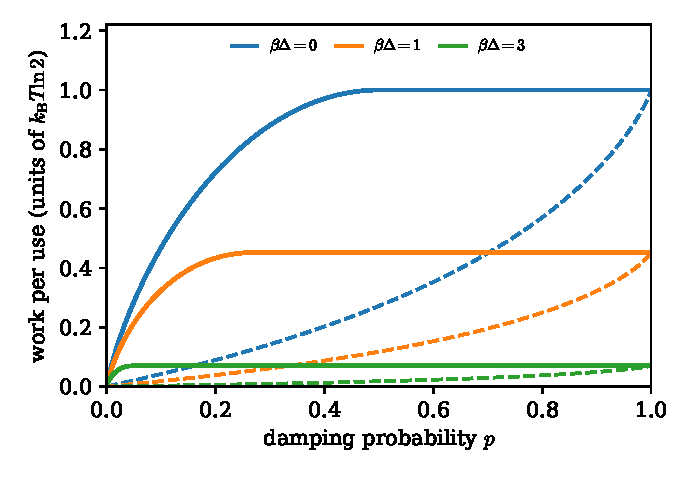
\includegraphics[width=0.62\linewidth]{fig-damping.pdf}
\caption{Work per use of amplitude damping with probability $p$, in real time (solid) and in batch (dashed), at three values of $\beta\Delta$. The curves meet only at $p=0$ and at full reset, $p=1$. Beyond $p=1/(1+e^{\beta\Delta})$ the real-time cost equals the cost of a full reset.}
\label{sw:fig:damping}
\end{figure}

The real-time formula has a striking consequence. Maximizing $h(y)-\beta\Delta y/\ln 2$ over all $y$ gives $y=1/(1+e^{\beta\Delta})$ and the value $\log_2(1+e^{-\beta\Delta})$, which is the cost of a full reset. So once $p\ge1/(1+e^{\beta\Delta})$, a partial reset costs exactly as much as a full one in real time (Figure~\ref{sw:fig:damping}). In batch, the cost of a partial reset rises smoothly to that value and reaches it only at $p=1$.

\paragraph{A finite example.} At one point the real-time cost can be met by a small explicit device. Take $p=1/2$ and $\beta\Delta=\ln2$. Since $p\ge1/(1+e^{\beta\Delta})$, the real-time cost is that of a full reset, $\log_2(3/2)$ bits or about $0.585\,\Delta$ per use, and the device never has to recover anything. Before the first input it prepares one ground-state qubit of gap $\Delta$ per use, and in round $t$ it applies the conserving rotation $|10\rangle\mapsto(|10\rangle+|01\rangle)/\sqrt2$ to the input and the $t$-th prepared qubit. The preparation uses only ordinary thermal qubits. Pool the $n$ memory qubits, initially thermal, with $R$ reservoir qubits of the same gap, and let a battery qubit of gap $w\Delta$ start excited. The $k$-excitation shell of the pool has dimension $\binom{R+n}{k}$. Whenever $\binom{R}{k+w}\ge\binom{R+n}{k}$, one energy-conserving permutation moves the whole shell onto states with every memory in its ground state, the reservoir in shell $k+w$ and the battery lowered; the other shells are left alone. The ratio $\binom{R}{k+w}/\binom{R+n}{k}$ decreases in $k$, so the preparation fails exactly on an upper tail of $\mathrm{Bin}(R+n,1/3)$. Because it happens before any input, its failure probability bounds the error against every adaptive observer once, not once per round. After the last output each memory is swapped with a fresh thermal qubit of the same gap, which returns the controller exactly on every branch. Table~\ref{sw:tab:finite} gives exact values for $n=100$. With $R=n^2$ and $w=n\log_2(3/2)+O(\sqrt{\ln n})$ the error is at most $n^{-2}$ for $n\ge1000$, by Hoeffding's inequality. The preparation is one large nonlocal permutation, not an efficient circuit.

\begin{table}[t]
\centering
\begin{tabular}{rrrrr}
reservoir $R$ & qubits & work & per use & error at most\\\hline
2{,}000  & 2{,}208  & $118\Delta$ & $1.18\Delta$ & $0.00999$\\
10{,}000 & 10{,}208 & $70\Delta$  & $0.70\Delta$ & $0.00548$\\
50{,}000 & 50{,}208 & $63\Delta$  & $0.63\Delta$ & $0.00156$
\end{tabular}
\caption{Real-time amplitude damping with $p=1/2$ at $\beta\Delta=\ln2$, for $n=100$ uses; the asymptotic cost is $0.585\Delta$ per use. The qubit count includes the reservoir, 100 memories, 100 fresh thermal qubits for the final swaps, a 7-qubit round counter and the battery. The battery drops by the stated work with probability one minus the error and is otherwise untouched. Errors are exact binomial tails, rounded up.}
\label{sw:tab:finite}
\end{table}

\paragraph{A finite saving.} The same example shows the batch saving at a finite size. At $p=1/2$ and $\beta\Delta=\ln2$ the batch capacity is about $0.154\,\Delta$ per use, against $0.585\,\Delta$ in real time, but batch constructions approach it only slowly. Fix the error at $10^{-8}$, and allow the controller to lose at most $10^{-5}\Delta$ of free energy, the battery to end with at most $10^{-5}$ bits of entropy, and its mean energy to differ from the nominal level by at most $10^{-5}\Delta$. Every real-time implementation of $234$ uses then has nominal work above $132.109\,\Delta$. This is~\eqref{sw:eq:converse} with the estimate of Appendix~\ref{sw:app:invertible} at the input with excited population $16/25$, where $\|(\Phi^c)^{-1}\|_\diamond=3$, less the three budgets. Only product inputs are used, so the bound also holds under the batch error criterion. A batch implementation does better. It prepares $234$ pure environment qubits for $137\Delta$ and runs the conserving partial swap of the real-time device. Before releasing the outputs it swaps the used environment into one of $32$ fresh thermal copies, chosen by a thermal five-qubit register, and then locates it again from the outputs, a position decoder as in~\cite[Sec.~7]{FBB21}. This purifies the register and returns $5\Delta$, so the nominal work is $137\Delta-5\Delta=132\Delta$, with error below $8.71\times10^{-9}$. At $256$ uses the same construction prepares the environments for $150\Delta$ and returns $11\Delta$ from $2^{11}$ positions: nominal work $139\Delta$ against a real-time bound of $144.53\Delta$, a saving above $5.5\Delta$. The saving needs the error: at zero error, the estimate of Appendix~\ref{sw:app:invertible} applied to the whole block gives a batch device the same bound as real time, as in the exact row of Theorem~\ref{sw:thm:werner}. The reservoirs that run the preparation and the refund are astronomically large, so this certifies that waiting saves work at a definite finite size, not that the saving is practical.

\subsection{The Werner--Holevo channel}\label{sw:sec:werner}

The Werner--Holevo channel $W(\rho)=(\Tr(\rho)\,I-\rho^T)/2$ on a qutrit is the standard example of a unital channel that is not a mixture of unitaries~\cite{LandauStreater93}. It is not even factorizable~\cite[Ex.~3.1]{HaagerupMusat11}, so it is not a limit of noisy operations. Its Choi state is the normalized projector onto the antisymmetric subspace of two qutrits. The isometry
\[
V|i\rangle=\tfrac{1}{\sqrt2}\sum_{j,k}\epsilon_{ijk}\,|j\rangle|k\rangle
\]
is a Stinespring dilation in which output and environment play symmetric roles, so $W$ is its own complementary channel. And $W$ is invertible, with $W^{-1}(Y)=\Tr(Y)\,I-2Y^T$.

\begin{proof}[Proof of Theorem~\ref{sw:thm:werner}]
\emph{Real time.} By Lemma~\ref{sw:lem:invertible}, $s_\rho(W)=S(W(\rho))$, which is at most $\log_2 3$ and equals it at $\rho=I/3$; so $\Trt(W)=\log_23$. Every exact real-time round on half of a maximally entangled pair adds exactly $\log_2 3$ bits of entropy to the device, whatever the device did before, and Lemma~\ref{sw:lem:accounting} gives $w\ge n\log_23$. With an information battery, a device that applies $V$ with one pure qutrit of the battery per round, and swaps the used qutrit into a thermal cell, attains this. At error $\varepsilon$ the same argument, run through the bounded inverse and continuity of conditional entropy on the nine-dimensional system $QO$, gives
\[
w\ \ge\ \sum_{t=1}^n\bigl[\log_2 3-g_9\bigl(\min\{1,10\sqrt{\varepsilon}\}\bigr)\bigr]_+,\qquad g_D(t)=2t\log_2 D+(1+t)\,h\bigl(t/(1+t)\bigr),
\]
which is $n\log_2 3-O(\log n)$ at $\varepsilon=n^{-2}$.

\emph{Batch.} The batch rate is zero by the theorem of Faist, Berta and Brand\~ao, since $\Tcap(W)=0$ for a unital channel at zero Hamiltonian~\cite{FBB21}. In the proof of their thermal-operation construction~\cite[Thm.~7.1]{FBB21}, the error at a fixed typicality tolerance $\delta$ is $\mathrm{poly}(n)\,e^{-n\eta/2}$, with an exponent $\eta=\eta(\delta)>0$ that tends to zero with $\delta$ (their Eqs.~(7.30), (7.36) and~(7.39)), and the work per copy tends to the capacity as $n\to\infty$ and then $\delta\to0$. At each fixed $\delta$ the error is below $n^{-2}$ for all large $n$, so letting $\delta$ step down to zero slowly enough, each step taken only once $n$ exceeds the threshold for the new value, gives work $o(n)$ at error $n^{-2}$. For exact batch implementation, the joint output-reference state must lie in the support of the $n$-fold antisymmetric projector, on which the partial trace acts as the invertible map $W^{\otimes n}$. The argument of Lemma~\ref{sw:lem:invertible} then forces $w\ge n\log_23$, attained by the same pure qutrits.
\end{proof}

No exact implementation can end with a sharp mechanical battery: each exact round triples the rank of the device, so if the controller returns, a battery that starts pure must end with rank at least $3^n$. This is why the exact entries of Theorem~\ref{sw:thm:werner} are stated for free energy.

The bound in the real-time part is measurable. Let $\delta$ be the average probability that the output and the reference of a round fail a two-outcome test for the antisymmetric subspace. Any real-time implementation, of any size and with any memory, then draws at least $n[\log_2 3-g_9(\min\{1,10\sqrt{\delta}\})]_+$ bits of free energy (Appendix~\ref{sw:app:werner}). We return to this in Section~\ref{sw:sec:discussion}.

The zero-error obstruction of Theorem~\ref{sw:thm:werner} holds for every extreme channel. A channel is extreme in the convex set of channels when the products $A_i^*A_j$ of its minimal Kraus operators are linearly independent~\cite{Choi75}; Werner--Holevo and amplitude damping with $0<p<1$ are examples.

\begin{proposition}[At zero error, waiting saves nothing for extreme channels]\label{sw:prop:extreme}
Let $\Phi$ be extreme with complementary channel $\Phi^c$, and let
\[
a_\beta(\Phi)=\max_\rho\Bigl[S(\Phi^c(\rho))+\tfrac{\beta}{\ln2}\Tr H\bigl(\Phi(\rho)-\rho\bigr)\Bigr].
\]
Every implementation of $n$ uses with zero error, in batch or in real time, draws at least $n\,a_\beta(\Phi)-o(n)$ bits of free energy from its battery and controller. For extreme channels $a_\beta(\Phi)=\Trt(\Phi)$, so at zero error a batch device pays the full real-time rate.
\end{proposition}

The proof is in Appendix~\ref{sw:app:extreme}: extremality makes the branches of any exact implementation orthogonal, so the device's entropy rises by exactly the entropy of the complementary output, whatever its initial state.

For amplitude damping at $p=1/2$ and $\beta\Delta=\ln2$, the asymptotic separation between $0.585\,\Delta$ per use in real time and the batch capacity $0.154\,\Delta$ therefore exists only because some error is tolerated. The finite constructions of Section~\ref{sw:sec:classical} certify smaller savings, at their stated block sizes and error budgets.

\subsection{What is free}\label{sw:sec:free}

A \emph{thermal operation} at $(H,\beta)$ is a channel $\rho\mapsto\Tr_BU(\rho\otimes\gamma_B)U^*$, where the bath $B$ (not the battery of Section~\ref{sw:sec:setting}) is finite-dimensional with an arbitrary Hamiltonian $H_B$, $\gamma_B$ is its Gibbs state at the same $\beta$, and $U$ commutes exactly with $H\otimes I+I\otimes H_B$~\cite{Janzing00,HorodeckiOppenheim13,Brandao13,vomEnde22,LieEtAl26}. We impose no large-bath conditions. The set is not closed~\cite{vomEnde22}, and by a limit of thermal operations we mean a point of its closure. \emph{Enhanced thermal operations} are the time-covariant channels that preserve $\gamma$~\cite{Cwiklinski15}.

Which processes are free? We call a process \emph{free in batch} (\emph{in real time}) if its optimal batch (real-time) work rate is zero, at vanishing error. Thermal operations, energy-conserving unitaries with a Gibbs bath, are the standard model of free dynamics~\cite{Janzing00,HorodeckiOppenheim13,Brandao13}. They preserve the Gibbs state and commute with time evolution~\cite{Lostaglio15}. Gibbs-preserving maps~\cite{Janzing00,FDOR15,FR18} are strictly more powerful: they can even create coherence between energy levels~\cite{FOR15}. The time-covariant ones, called enhanced thermal operations~\cite{Cwiklinski15}, coincide with the closure of the thermal operations for a qubit~\cite{Cwiklinski15,vomEnde22}, but not for a qutrit~\cite{Cwiklinski15,DingFengHu21}. By the theorem of Faist, Berta and Brand\~ao, a time-covariant process is free in batch exactly when it is an enhanced thermal operation (see below). In real time the answer is the thermal operations.

\begin{theorem}[What is free in real time]\label{sw:thm:free}
Let $\Phi$ be any channel on a system with Hamiltonian $H$, at any temperature. Then $\Trt(\Phi)=0$ if and only if $\Phi$ lies in the closure of the thermal operations.
\end{theorem}

Lie, Son, Boes, Ng and Wilming showed that a channel that fixes the Gibbs state is a thermal operation exactly when some dilation, with no energy conservation or thermal bath assumed, also leaves its environment unchanged when the input is the Gibbs state; energy conservation, a thermal bath and time covariance then follow~\cite[Prop.~4]{LieEtAl26}. Theorem~\ref{sw:thm:free} is a robust, work-cost form of their criterion. As in their exact case, zero cost forces time covariance and only the Gibbs input matters; here the bounds do not depend on the size of the bath, and this is what characterizes the closure.

So the enhanced thermal operations that are not limits of thermal operations are exactly the time-covariant processes that are free in batch but cost work in real time. This set is known to be nonempty. At zero Hamiltonian it contains the Werner--Holevo channel, which is not factorizable~\cite[Ex.~3.1]{HaagerupMusat11} and which Faist, Oppenheim and Renner cite as a unital map that is not a thermal operation~\cite{FOR15}, and for an equally spaced qutrit a channel of Ding, Ding and Hu~\cite{DingFengHu21}. We price both: $\log_23$ bits per use for the first (Theorem~\ref{sw:thm:werner}), and an explicit positive cost, at every gap ratio and temperature, for a family that contains the second (Proposition~\ref{sw:prop:qutrit}). For that family a single input state already separates the channel from every limit of thermal operations, with no assumption on the bath; Ding, Ding and Hu proved this for equally spaced levels, under assumptions on the bath and the temperature.

\paragraph{Batch.} For time-covariant $\Phi$ the batch cost is $\Tcap(\Phi)=\max_\rho[D(\Phi(\rho)\|\gamma)-D(\rho\|\gamma)]$, in relative-entropy form. The value at $\rho=\gamma$ is $D(\Phi(\gamma)\|\gamma)\ge0$, and by monotonicity of relative entropy every value is at most zero when $\Phi(\gamma)=\gamma$. So $\Tcap(\Phi)=0$ exactly when $\Phi$ is an enhanced thermal operation, and by the theorem of Faist, Berta and Brand\~ao such a process can be run in batch at vanishing work per use~\cite{FBB21}. This is a direct consequence of their work; we record it only for contrast. Faist, Oppenheim and Renner ask whether thermal operations aided by a time reference can do everything Gibbs-preserving maps can~\cite{FOR15}, and Tajima and Takagi showed that for some Gibbs-preserving maps no finite amount of coherence suffices~\cite{TajimaTakagi25}. For a device that carries its own phase reference and must return it, a Gibbs-preserving channel is free in batch exactly when its energy change lies in the span of the products of its Kraus operators; some non-covariant Gibbs-preserving channels are free and others cost work (Appendix~\ref{app:batch}).

\paragraph{Real time: thermal operations are free.} Let $\Phi$ be a thermal operation with bath $(H_B,\gamma_B)$. Its dilation is an exact extension in Definition~\ref{sw:def:rtcost}, with the bath purifier as $F$. Energy conservation and the Gibbs identity give, for every input,
\[
s_\rho(\Phi)+\tfrac{\beta}{\ln2}\Tr H\bigl(\Phi(\rho)-\rho\bigr)\ \le\ -D\bigl(\Gamma(\rho)\,\big\|\,\gamma_B\bigr)\ \le\ 0,
\]
where $\Gamma(\rho)$ is the bath output. So $\Trt(\Phi)=0$. If $\Phi$ is only a limit of thermal operations $\Phi_k$, the dilation of $\Phi_k$ is a feasible extension for $\Phi$ at error $\varepsilon$ once $\Phi_k$ is $\varepsilon$-close to $\Phi$, so the same bound holds for $s_{\rho,\varepsilon}(\Phi)$ up to an energy correction of order $\beta\varepsilon\,\mathrm{span}(H)$. Letting $\varepsilon\to0$, every limit of thermal operations has zero real-time cost as well. Operationally this is the obvious statement that a device using one fresh thermal bath per round runs a thermal operation in real time at no cost.

\paragraph{Real time: only thermal operations are free.} The converse is the substance of Theorem~\ref{sw:thm:free}. For baths of bounded size it follows from compactness and the exact characterization of Lie et al.~\cite{LieEtAl26}, but a small real-time cost may be achieved only with baths of unbounded size and arbitrarily small eigenvalues. We prove it in four steps (Appendix~\ref{sw:app:zero-set}).
\begin{enumerate}[label=(\roman*)]
\item Since $\Trt(\Phi)\ge D(\Phi(\gamma)\|\gamma)$, zero cost forces $\Phi(\gamma)=\gamma$. It also supplies dilations whose \emph{Gibbs defect} $G=D\bigl(U(\gamma\otimes\tau)U^*\,\big\|\,\gamma\otimes\omega\bigr)$ tends to zero, where $\omega$ is the bath output on input $\gamma$. The defect is the relative entropy between the joint output and the product of the Gibbs state with the bath output; it vanishes exactly for the equilibrating dilations of Lie et al., up to a unitary on the bath.
\item A small Gibbs defect forces time covariance. This is a robust form of Proposition~4 of~\cite{LieEtAl26}: the dilation nearly commutes with $(\gamma\otimes\tau)^{iz}$, the time evolution of $H+H_B$ with $H_B=-\beta^{-1}\ln\tau$, with a bound that involves neither the bath dimension nor its smallest eigenvalue.
\item A replacement theorem turns any dilation of a time-covariant channel with small defect $G$ into a finite thermal operation within $c_{H,\beta}\,G^{1/(6\max\{1,r\})}$ in diamond norm, where $r$ is the number of rationally independent energy gaps of $H$. The new thermal operation generally has a different bath.
\item Irrational energy gaps are approximated by commensurate ones with the same integer labels, and a finite thermal lattice absorbs the difference so that the original Hamiltonian is conserved exactly. This handles the accidental gap coincidences at which thermal operations depend discontinuously on $H$~\cite[Sec.~III]{vomEnde22}. No external phase reference is used.
\end{enumerate}
As in the exact criterion of Lie et al., only the Gibbs input matters: $\Phi$ is a limit of thermal operations exactly when $\Phi(\gamma)=\gamma$ and the real-time entropy cost at the Gibbs input vanishes. Lie et al.\ also observe that an enhanced thermal operation outside the thermal operations must change its environment even at the Gibbs input, so its environment must hold non-equilibrium free energy, which may be depleted~\cite{LieEtAl26}. The real-time entropy cost $s_\gamma(\Phi)$ is the least such change, and in real time it is paid in work.

Two remarks on the controller. The controller acts as a catalyst that is returned only at the end and may be correlated with past outputs; it does not enlarge the free set, because those correlations only add to the cost in Lemma~\ref{sw:lem:accounting} and its free energy must return up to $o(n)$, which also excludes the embezzlement that a catalyst returned only approximately would otherwise allow~\cite{FOR15}. And since the lower bound of Section~\ref{sw:sec:law} holds for any controller, Theorem~\ref{sw:thm:free} bears on the time-reference question of Faist, Oppenheim and Renner~\cite{FOR15}: a phase reference that the device must return, up to $o(n)$ free energy, cannot make a non-covariant Gibbs-preserving map free in real time. A reference that is used up and paid for is not covered.

\paragraph{A clock that returns cannot help.} If the controller returns exactly, as in our constructions of time-covariant channels, and the battery is stationary, a non-covariant channel cannot be run at vanishing error, whatever work is spent~\cite{MarvianSpekkens19,LostaglioMuller19}. The following proposition makes this quantitative.

\begin{proposition}[A returning clock]\label{sw:prop:clock}
Suppose the controller returns exactly to $\alpha_C$, independent of all other systems, and the battery is stationary. Let $J_\Phi$ be the normalized Choi state of $\Phi$ and $G=H_O-H_I^T$, where $H_I=H_O=H$ act on the input and output. Then, in real time or in batch and whatever work is drawn, every implementation of $n$ uses of $\Phi$ has error at least
\[
\tfrac14\sup_t\bigl\|J_\Phi-e^{-\mathrm itG}J_\Phi e^{\mathrm itG}\bigr\|_1,
\]
which is positive exactly when $\Phi$ is not time-covariant. For the Hadamard gate on a qubit with $H=E|1\rangle\langle1|$ the error is at least $1-2^{-n}\binom{n}{\lfloor n/2\rfloor}$, which tends to one.
\end{proposition}

\begin{proof}
Fix an observer whose inputs, together with the systems it keeps, are invariant under time evolution; the initial reservoir states are invariant too, and so is the battery's, because it is stationary. Composing every operation of the device, including its final clean-up, and tracing out everything except the controller and a set $Y$ of systems we keep, gives a channel $\Lambda$ from $C$ to $CY$ that commutes with time evolution. Exact return means $\Lambda(\alpha)=\alpha\otimes\rho$. Write $x_t$ for a state evolved for time $t$. Covariance gives $\Lambda(\alpha_t)=\alpha_t\otimes\rho_t$, and since fidelity does not decrease under $\Lambda$ and is multiplicative on products, $f(\alpha,\alpha_t)\le f(\alpha,\alpha_t)f(\rho,\rho_t)$. For small $t$ the fidelity $f(\alpha,\alpha_t)$ is positive, so $\rho_t=\rho$, and by the group law this holds for every $t$. So the final state of everything we keep is invariant in time: a controller cannot pass on asymmetry and keep it, which is the no-broadcasting theorem for asymmetry~\cite{MarvianSpekkens19,LostaglioMuller19}.

For the first bound, let the observer send half of a maximally entangled state in the first round, and $|0\rangle$ in every later round, and keep the other half as a reference with Hamiltonian $-H^T$, so that the pair is invariant. The first output and the reference end in a state $J'$ that commutes with $G$, so $\|J_\Phi-e^{-\mathrm itG}J_\Phi e^{\mathrm itG}\|_1\le2\|J_\Phi-J'\|_1$ for every $t$, and the observer distinguishes $J'$ from $J_\Phi$ with advantage $\tfrac12\|J_\Phi-J'\|_1$. For the Hadamard gate, send $|0\rangle$ in every round. The outputs end in a state that commutes with the total energy, while the ideal output $|+\rangle^{\otimes n}$ has weight $2^{-n}\binom nk$ in the sector with $k$ excitations. So the real output passes the test for $|+\rangle^{\otimes n}$ with probability at most $\max_k2^{-n}\binom nk$, and the ideal one with probability one.
\end{proof}

The battery must be stationary. A battery in a broad superposition of energy levels is a phase reference of its own, and the device may spend it while the controller returns exactly. Let the battery be a ladder with spacing $E$, prepared in a sine-shaped wave packet on $L$ consecutive levels with $n+1$ empty levels on each side, and let each use apply the Hadamard gate to every pair $\{|0\rangle|q\rangle,|1\rangle|q-1\rangle\}$ of equal total energy, and the identity on the two unpaired states at the edges. This unitary conserves energy. Because the packet barely changes when it is shifted by one level, each use acts as the Hadamard gate up to $\pi/(\sqrt2(L+1))$ in strategy distance, whatever the observer does. With $L=n^3$ and a trivial controller, $n$ uses have error $O(n^{-2})$, while the battery's entropy changes by at most $\log_2(L+2n+2)=o(n)$. The battery's coherence is spent, not broadcast, so this is consistent with the no-broadcasting theorem; it shows that every initial store of asymmetry, a coherent work store included, must be counted as part of the controller.

\paragraph{A clock that returns approximately.} Theorem~\ref{sw:thm:clock} relaxes the return condition. A controller \emph{returns approximately} if, uniformly over observers, its final joint state with all other systems is within $\eta_n\to0$ in trace distance of $\alpha_C$ tensored with their final state, and its mean energy and its entropy change by $o(n)$. This is the return condition of our lower bounds, with closeness of the joint state added. Trace-distance closeness alone would not suffice: a broad reference can hand over energy of order $n$ while staying close to its initial state, and would then act as a second battery. The controller may start with any declared amount of phase reference.

\begin{theorem}[A clock that returns approximately]\label{sw:thm:clock}
Let $\Phi$ be any channel. Suppose the controller need only return approximately: its final joint state with everything else is close to its initial state tensored with the rest, and its mean energy and its entropy change by $o(n)$. Then the optimal real-time work per use at vanishing error is $\kB T\ln2\,\Trt(\Phi)$, with deterministic work. For a unitary $U$ it is exactly the largest eigenvalue of $U^*HU-H$, and the battery reaches its target on every branch. If $U$ is not time-covariant, the heat baths of any such implementation with deterministic work must have a total energy range that grows faster than $n$.
\end{theorem}

Faist, Berta and Brand\~ao leave open whether thermal operations can implement every i.i.d.\ channel that is not time-covariant at its thermodynamic capacity, and expect this to need a very large amount of coherence, as the reverse Shannon theorem needs embezzling states~\cite{FBB19},~\cite[Sec.~9]{FBB21}. Theorem~\ref{sw:thm:clock} settles the real-time analogue of this question: a clock that returns approximately runs every channel at the optimal real-time rate, and the coherence it needs is indeed large. In batch, a clock that must return in the same sense, which rules out embezzlement, cannot always reach the capacity: for qubit dephasing in the $X$ basis, batch costs as much as real time, more than the capacity, and the batch cost of every channel with a returned clock is given in Appendix~\ref{app:batch}. The coherence is invested, not consumed. The operating work is the same formula, while for a gate the clock pays in capital~\cite{ChiribellaYangRenner21,TSS20} and the baths in energy range, and the controller's energy comes back only on average, not branch by branch (Appendix~\ref{app:batch}). Channels that are not gates can need far less: a Gibbs-preserving qubit channel that only creates coherence runs in batch at its capacity, zero, with a clock whose energy spreads like $\sqrt n$ (Appendix~\ref{app:batch}).

The lower half of Theorem~\ref{sw:thm:clock} is the bound of Section~\ref{sw:sec:law}, which uses neither time covariance nor exact return. The construction (Appendix~\ref{sw:app:clock}) rests on one primitive. Let $D=U^*HU-H$, $w$ its largest eigenvalue and $B=wI-D\ge0$. A thermal qubit with a large gap $M$ can absorb the energy $B$ by a rare excitation: a rotation between the payload and this qubit, by the angle whose sine is $\sqrt{B/M}$, changes the payload channel by only $O(\|B\|/M)$, yet the qubit takes up exactly the input-dependent part of the energy change, on average. What remains is the constant $w$, which a sharp battery supplies. Lifting the whole contact with a phase reference makes it conserve energy exactly, and the reference's energy then drifts by $O(1/M)$ as an operator, whatever the input. For the Hadamard gate on a qubit with $H=E|1\rangle\langle1|$, this gives work exactly $nE/\sqrt2$, with error and return error $O(n^{-3})$. For a general channel the same primitive is applied to a dilation whose bath carries the Hamiltonian $-\beta^{-1}\ln\zeta$, with $\zeta$ the bath state at the worst input. This turns the bath's entropy into energy, so one operator inequality handles the entropy and energy terms together. The bath copies are prepared in their source state, and everything used to prepare them is returned, by the finite-source module of Appendix~\ref{app:module}, applied with one slot.

The energy-conserving lift and the reusable reference go back to {\AA}berg~\cite{Aberg14}. Repaying a reference's drift with work is due to Korzekwa, Lostaglio, Oppenheim and Jennings~\cite{KLOJ16}, and forming coherent sources at their free-energy cost to~\cite{Brandao13,KLOJ16}. The rare-excitation primitive and the work rate for every channel appear to be new. The bound on the baths' range is an argument of Wigner--Araki--Yanase type, of the kind that bounds the energy and coherence a reference needs to implement a gate~\cite{ChiribellaYangRenner21,TSS20}; what is new is that, with deterministic work and a controller that returns, it falls on the heat baths. Faist, Berta and Brand\~ao already observed that for such channels the environment must coherently compensate the energy differences between inputs~\cite{FBB19}; the bound makes this quantitative.

\paragraph{The clock is expensive.} Theorem~\ref{sw:thm:clock} makes the operating work the formula, but the clock is not cheap. Unlike a circuit acting on one register, whose energy requirement need not grow with its depth~\cite{ChiribellaYangRenner21}, $n$ uses on fresh systems call for $n$ times the asymmetry. In Appendix~\ref{app:batch} we show that, for a gate, its initial free energy must grow at least like $n/(\varepsilon+\eta)$, where $\eta$ is the return error, a quantitative form of the trade-off between disturbing a reference and the asymmetry it can impart~\cite{MarvianSpekkens19}, that the range of its baths and the strength of their interactions must grow at least like $n/\sqrt\varepsilon$, and that its energy comes back only on average, through a lottery of rare large transfers.

At zero Hamiltonian a thermal operation is a mixture of noisy operations, unitaries acting with a maximally mixed bath~\cite{HHO03}. Lie et al.\ note that these mixtures are the strongly factorizable channels, and show that these are exactly the unital channels with an equilibrating dilation~\cite[Eq.~(14)]{LieEtAl26}, and their closure is the closure of the channels that factor through a finite-dimensional algebra with a faithful trace~\cite{MullerHermesPerry,Douglas26closed}. Thus at zero Hamiltonian Theorem~\ref{sw:thm:free} identifies real-time freeness with the closure of finite-dimensional factorizability, as in our earlier work~\cite{Memory}. The closure is needed: a channel can be a limit of finitely factorizable channels without factoring through any finite-dimensional algebra~\cite{MusatRordam}.

\paragraph{The gap.} For a qubit, enhanced thermal operations coincide with the closure of the thermal operations~\cite{Cwiklinski15},~\cite[Thm.~10]{vomEnde22}. For a qutrit they do not, already for state transitions: exactly~\cite{Cwiklinski15} and approximately~\cite{DingFengHu21}. By Theorem~\ref{sw:thm:free}, the difference is exactly the set of time-covariant processes that are free in batch but cost work in real time. At zero Hamiltonian it contains the Werner--Holevo channel, at a cost of $\log_2 3$ bits per use. At nonzero Hamiltonian it contains the following qutrit channels.

\begin{proposition}[A Gibbs-preserving process that is not free in real time]\label{sw:prop:qutrit}
Let $H=\mathrm{diag}(0,E_1,E_2)$ with $0<E_1<E_2$, let $\lambda=e^{-\beta E_2}$, and let $\Phi$ have Kraus operators $\mathrm{diag}(\sqrt{1-\lambda},1,0)$, $\sqrt\lambda\,|2\rangle\langle0|$ and $|0\rangle\langle2|$. Then $\Phi$ is an enhanced thermal operation, so $\Tcap(\Phi)=0$, but
\[
\Trt(\Phi)\ \ge\ g_1\log_2\frac{1}{1-g_2}\ >\ 0,
\]
where $(g_0,g_1,g_2)$ are the Gibbs populations. Moreover, for the input $\psi_0=(|0\rangle+|1\rangle)/\sqrt2$ and every limit of thermal operations $\Theta$,
\[
\tfrac12\bigl\|\Theta(\psi_0)-\Phi(\psi_0)\bigr\|_1\ \ge\ \delta(\lambda)=\frac{(1-\lambda)\Delta_\lambda^2}{4(1-\lambda)\Delta_\lambda+2\lambda\bigl(1+2\sqrt{1-\lambda}\bigr)},\qquad\Delta_\lambda=\sqrt{1-\lambda}-(1-\lambda)>0.
\]
In particular $\Phi$ is at half diamond distance at least $\max\{\delta(\lambda),u^2/(2c^2)\}$ from the closure of the thermal operations, where $u=g_1g_2$ and $c=2+6u/\sqrt{1-\lambda}$.
\end{proposition}

The channel leaves level $1$ untouched, resets level $2$ to the ground state, and excites the ground state with probability $\lambda$, while keeping the coherence between levels $0$ and $1$ as large as positivity allows. The proof shows that the bath must end in orthogonal states after leaving level $1$ alone and after resetting level $2$. At the Gibbs input this forces correlations between bath and output worth at least $g_1\log_2\frac1{1-g_2}$ bits.

For equally spaced levels this is the enhanced thermal operation that Ding, Ding and Hu use (their Eq.~(11) with the transition matrix of their Eq.~(17)). It saturates the coherence bounds of~\cite{Cwiklinski15,Lostaglio15}. They proved that its output on $\psi_0$ cannot be approximated by any thermal operation acting on that input~\cite{DingFengHu21}, for equally spaced levels, bath degeneracies that grow with energy as in~\cite{HorodeckiOppenheim13}, and a range of temperatures. Proposition~\ref{sw:prop:qutrit} removes all three assumptions and bounds the trace distance explicitly. Their bound is stated for perturbations of transition probabilities, so the two constants are not directly comparable.

The single-input bound rests on a law for thermal operations that may be of independent interest (Lemma~\ref{sw:lem:coherence}). If a thermal operation moves the ground state to level $2$ with probability $T_{20}$, then $T_{20}\le\lambda$, and the coherence it keeps between levels $0$ and $1$ is at most $\frac12\bigl[1-\lambda+\sqrt{\lambda(\lambda-T_{20})}\bigr]$. The reason is that the bath can give up the energy $E_2$ only from states of total Gibbs weight at most $\lambda$. Moving the full probability $\lambda$ to level $2$ therefore forces an all-or-nothing transfer on those states, while $\Phi$ acts as if every state of the bath contributed the same partial amplitude $\sqrt\lambda$. With $T_{20}=\lambda$, $\Phi$ keeps the coherence $\sqrt{1-\lambda}/2$, above the bound by $\Delta_\lambda/2$.

\subsection{Undecidability}\label{sw:sec:undecidable}

Our last result concerns generalized dephasing channels, also called Schur multiplier channels: $\Phi(\rho)=M\circ\rho$, the entrywise product with a positive semidefinite matrix $M$ that has unit diagonal.

\begin{theorem}[Undecidability]\label{sw:thm:undecidable}
There is a dimension $d_0$ with the following property. For every $d\ge d_0$, every Hamiltonian on $\mathbb C^d$ that is diagonal in the dephasing basis and every temperature, no algorithm decides whether a generalized dephasing channel on $\mathbb C^d$ with cyclotomic entries is free in real time. The set of such channels that are free is not recursively enumerable.
\end{theorem}

By Theorem~\ref{sw:thm:free}, free in real time means a limit of thermal operations; on these channels the easy direction of Theorem~\ref{sw:thm:free} is enough, because the other direction is supplied by the zero-Hamiltonian closure theorem of our earlier preprint~\cite[Thm.~3.2(a)]{Memory} (Step~1 of the proof below). In batch the same question is trivial: a generalized dephasing channel preserves every energy population, hence the Gibbs state, so it is always free in batch. Our earlier work showed that the zero-Hamiltonian question is undecidable when the dimension may grow~\cite{Flagship}; Theorem~\ref{sw:thm:undecidable} settles the fixed-dimension question left open there.

On dephasing channels the Hamiltonian and the temperature drop out. Being free in real time becomes a question about which Gram matrices of unitaries finite-dimensional algebras can approximate, and that question is undecidable at a fixed size by the work of Fu, Miller and Slofstra.

\begin{proof}[Proof of Theorem~\ref{sw:thm:undecidable}]
\emph{Step 1: on dephasing channels, free means a limit of finitely factorizable channels.} Let $\Phi(\rho)=M\circ\rho$ be a generalized dephasing channel, and let the Hamiltonian be diagonal in the same basis. Then $\Phi$ preserves every energy population, so the energy term vanishes and $\Trt(\Phi)=\sup_\rho s_\rho(\Phi)$, the zero-Hamiltonian purity cost of our earlier work. That cost vanishes exactly when $\Phi$ is a limit of channels that factor through finite-dimensional algebras with a faithful trace~\cite[Thm.~3.2(a)]{Memory},~\cite{Douglas26closed}. For dephasing channels these are the limits of channels with $M_{ij}=\tau(u_j^*u_i)$ for unitaries $u_i$ in a finite-dimensional algebra $\mathcal N$ with faithful trace $\tau$~\cite{HaagerupMusat11,Musat25}. Each such channel is a thermal operation. Write $\mathcal N=\bigoplus_k M_{n_k}$ with $\tau=\sum_kw_k\tr_{n_k}$ (normalized traces), give the bath the Hamiltonian $H_B=\bigoplus_kE_kI_{n_k}$ with $e^{-\beta E_k}=w_k/n_k$, so that its Gibbs state is the density of $\tau$, and use $U=\sum_i|i\rangle\langle i|\otimes u_i$. This $U$ commutes with $H\otimes I+I\otimes H_B$, its bath starts in the Gibbs state, and it implements $\Phi$. (This is the dilation used for Schur multipliers in~\cite{HaagerupMusat11,LieEtAl26}, with the bath Hamiltonian read off from the trace as in~\cite{LieEtAl26}.) Conversely, every limit of thermal operations has zero real-time cost (Section~\ref{sw:sec:free}). So a dephasing channel is a limit of thermal operations exactly when it is a limit of finitely factorizable channels, at every temperature and for every Hamiltonian diagonal in its basis. This step does not use the hard direction of Theorem~\ref{sw:thm:free}; the direction it needs, from zero cost to a limit of finitely factorizable channels, is imported from~\cite[Thm.~3.2(a)]{Memory}.

\emph{Step 2: the reduction.}
\begin{enumerate}[label=(\alph*), leftmargin=*]
\item For a recursively enumerable but not recursive set $X$, Fu, Miller and Slofstra give a number $N$ of questions, eight answers, and a computable map from $n$ to finite lists of real tables with cyclotomic entries: if $n\in X$ none of them is a commuting-operator correlation, and if $n\notin X$ one of them is an approximately quantum synchronous correlation~\cite[Thm.~7.2]{FMS}. Exact tests discard every table that is not a synchronous correlation (Appendix~\ref{sw:app:fixeddim}).
\item Approximately quantum synchronous correlations are exactly those realized by projections in an ultrapower of the hyperfinite factor~\cite{KPS18}.
\item The construction of Musat and R{\o}rdam turns such projections into unitaries in the same algebra with a prescribed Gram matrix~\cite{MusatRordam}.
\item The corresponding dephasing channel on $\mathbb C^{d_0}$, $d_0=16N+1$ (the identity, the $8N$ symmetries $2p_j-1$ and the $8N$ unitaries $(2p_j-1+i)/\sqrt2$), is a limit of finitely factorizable channels exactly when its Gram matrix is a limit of finite-dimensional ones~\cite{Musat25}. Repeating indices embeds it in every dimension $d\ge d_0$.
\end{enumerate}
The entries lie in cyclotomic fields: the construction of Fu, Miller and Slofstra uses sines and cosines of rational multiples of $\pi$ and finite group-algebra coefficients~\cite[Sec.~7, Thm.~7.2]{FMS}, and the transfer to unitaries adds only $i$ and $\sqrt2$. The field grows with $n$; no fixed number field is claimed. So each channel is a finite, exact input. Appendix~\ref{sw:app:fixeddim} gives the reduction in full: the faithful Gram transfer, the exact filters on the tables, and the padding to larger dimensions. Program $n$ never halts exactly when some channel in its list is free; when it halts, no channel in the list is even factorizable. If the free channels were recursively enumerable, the non-halting programs would be too, which is impossible.\footnote{The reduction asks whether at least one channel in a finite list is free, so it is a disjunctive truth-table reduction from the complement of the halting problem rather than a many-one reduction. The dimension $d_0=16N+1$ is not explicit, because Fu, Miller and Slofstra do not give $N$ explicitly.}
\end{proof}

